%% Paper 2 - Results in Engineering (Elsevier), Special Issue 335088
%% "Emerging Trends in Computational Science and Engineering".
%% Chuyen tu ban Springer sn-jnl: ../paper2_overleaf/main.tex (GIU LAI, dung neu phai doi tap chi).
%%
%% KHUNG VIET LAI cho cua "engineering" cua RINENG:
%%   scope noi ro "A clear engineering problem, system, or process must be addressed."
%%   -> bai duoc dat lai thanh BAI TOAN THIET KE mot he do duoi BA rang buoc ngan sach:
%%      (1) ngan sach chu thich, (2) ngan sach tinh toan, (3) dac ta do tin cay.
%%   Khong so lieu nao moi; chi doi thu tu uu tien va cach dat van de.
%%
%% >>> Bien dich bang pdfLaTeX.
\documentclass[preprint,12pt]{elsarticle}

\usepackage{amsmath,amssymb}
\usepackage{booktabs}
\graphicspath{{figures/}{./}}

\journal{Results in Engineering}

\begin{document}
\begin{frontmatter}

\title{Annotation-efficient design of an automated nuclei quantification system:
image-level counts match pixel-level masks at under one eighth of the labelling cost}

%% Thu tu tac gia theo thoa thuan: Duong Viet Hang dung dau, Dinh Thi Thu Hiep lien he.
\author[uit]{Viet Hang Duong}
\ead{hangdv@uit.edu.vn}

\author[uit]{Thi Thu Hiep Dinh\corref{cor1}}
\ead{dinhthithuhiep1@gmail.com}
\cortext[cor1]{Corresponding author.}

\affiliation[uit]{organization={Faculty of Computer Science, University of Information Technology (UIT), VNU-HCM},
            city={Ho Chi Minh City},
            country={Vietnam}}

%% KHI RUT GON ABSTRACT, BON CUM SAU PHAI GIU (moi cum chan mot cach hieu sai, da bi cat 4 lan):
%%   "the same test set"        -> can cu cong bang cua so sanh 4 paradigm
%%   "require localisation"     -> giu luan diem hieu qua nhan, khong thanh khoe benchmark
%%   "full delineation"         -> 8x CHI dung voi mat na, khong dung voi nhan diem (14 phut)
%%   "sham-controlled"          -> bao hieu nhan qua, khong phai tuong quan
\begin{abstract}
Deploying an automated nuclei quantification system is limited in practice less by model capacity than by two
engineering constraints: the expert labour needed to annotate its training data, and the requirement that every
reported number carry a stated tolerance. Pixel-level annotation costs hours of expert time per image and scales
poorly to new tissues, organs or centres, yet most counting methods rely on segmentation, density estimation or
detection, implying that dense spatial supervision is a prerequisite for high accuracy. This paper tests that
assumption directly with a controlled experiment in which the network architecture, the data and the evaluation
protocol are held fixed while supervision type is the only variable. Given a single image-level count as its only
label, a 3.62M-parameter model achieved an $R^2$ of 0.918 on PanNuke and outperforms the surveyed representatives
of segmentation, density estimation and detection on the same counting task and the same test set, even though all
three require localisation labels. Comparing count supervision with mask supervision on PanNuke, NuInsSeg and
MoNuSeg, the sign of the difference reverses across datasets, so neither regime is consistently superior. On
PanNuke the advantage of mask supervision is statistically significant but bounded above by an equivalence test at
1.1\% of the mean nuclei per image, while count labels are at least eight times cheaper than full delineation.
Sham-controlled intervention experiments show that the model responds specifically to nuclear content, yet forms
its prediction by integrating evidence over the whole image rather than by localising individual instances. The
resulting counter runs in $6.0$\,ms on GPU and $46$\,ms on CPU, and organ-conditional conformal prediction
intervals attain the target coverage across all 19 tissue types. Dense spatial annotation is therefore not a
prerequisite for accurate nuclei counting.
\end{abstract}

\begin{highlights}
\item Count-only labels match pixel masks for nuclei counting on three public datasets
\item An equivalence test bounds the gap at 1.1\% of the mean nuclei per image, n = 2722
\item Image-level counts cost under one eighth of full pixel-level delineation
\item A 3.62M-parameter counter runs in 6 ms on GPU and 46 ms on CPU at 256x256
\item Organ-conditional conformal intervals hold target coverage in all 19 tissues
\end{highlights}

\begin{keyword}
nuclei counting \sep annotation cost \sep weak supervision \sep uncertainty quantification \sep
conformal prediction \sep measurement system design \sep computational pathology
\end{keyword}

\end{frontmatter}

%%============================================================%%
\section{Introduction}\label{sec:intro}

The number and density of cell nuclei are fundamental quantitative readouts in pathology, supporting the
assessment of proliferation, tumour grading and analysis of the tissue microenvironment. Most current deep
learning methods approach nuclei counting indirectly, by \emph{segmenting} or \emph{detecting} individual
nuclei and then deriving the count from that output. Although accurate, these methods require pixel-level or
instance-level annotation, which costs hours of expert time per image and scales poorly to new tissues, organs
or centres.

Seen as an engineering problem, building such a system in a new laboratory is governed less by model capacity
than by three budgets. The first is the \emph{annotation budget}: the expert labour that must be bought before
the first model can be trained, which is the dominant non-recurring cost and the one that has to be paid again
whenever the system is moved to a new organ, stain or centre. The second is the \emph{compute budget} at
inference time, which decides whether the system can run beside the scanner or only on dedicated hardware. The
third is a \emph{reliability specification}: an instrument that reports a number without a stated tolerance
cannot be placed inside a decision process, and a tolerance that holds on average but fails on particular
tissue types is not a usable specification either. This paper treats the choice of supervision as a design
decision taken under those three budgets, and measures what the cheapest option actually costs.

Underlying the current norm is an assumption that is rarely tested directly: that accurate counting requires the
model to be given the \emph{location} of each nucleus during training. While supervision by the image-level
object total alone (\emph{count-only}) has been studied extensively in crowd counting and in several other
object counting problems, nuclei counting in histopathology still relies mainly on spatial annotation such as
points or masks. The minimum level of supervision that nuclei counting actually requires therefore remains an
open question, and with it the size of the annotation budget that a deployment must plan for.

This paper answers that question with a \emph{controlled experiment}. The model architecture, the data and the
evaluation protocol are held fixed, and the single experimental variable is the type of supervision:
pixel-level masks, or one count label per image. Any observed difference is therefore attributable to
\emph{annotation}, not to model capacity.

The main contributions are as follows.
\begin{itemize}
\item A controlled study of how the level of supervision affects counting accuracy, across three independent
datasets and a single architecture. Neither regime is consistently superior \emph{across datasets}: the sign of
the difference reverses, and on the largest test set the margin held by mask supervision, although
statistically significant, is bounded above by an equivalence test at $1.1\%$ of the mean nuclei per image
(Section~\ref{sec:parity}).
\item A mechanistic analysis based on intervention experiments with area-matched sham controls: the prediction
depends specifically on nuclear content, but the response is sublinear and the density map barely localises
nuclei at all. Together these two observations narrow the set of mechanisms that can explain the result above
(Section~\ref{sec:fidelity}).
\item A comparison against representatives of three paradigms that use localisation labels (segmentation,
density estimation and detection) under the same data and the same evaluation protocol: the lightweight
count-only counter attains higher counting accuracy than all three in their common configurations, while the
detection paradigm degrades systematically in densely packed regions (Section~\ref{sec:paradigm}).
\item A characterisation of the resulting system against the three budgets above: the annotation cost of each
label type, the inference cost on GPU and CPU, the accuracy recovered per unit of label budget, and
distribution-free prediction intervals whose coverage is guaranteed not only on average but within every
tissue type (Section~\ref{sec:deploy}).
\end{itemize}

%%============================================================%%
\section{Related work}\label{sec:related}

\paragraph{Nuclei segmentation and detection.} U-Net~\cite{unet} and extensions such as
HoVer-Net~\cite{hovernet} and StarDist~\cite{stardist} achieve high segmentation accuracy on benchmarks such as
PanNuke~\cite{pannuke}; in these methods the count is a quantity derived from the segmentation output and the
training labels are pixel-level masks. The same holds for recent lightweight models for nuclei quantification,
whether distilled from a pathology foundation model~\cite{distillfm} or built on specialised multi-head
architectures~\cite{kongnet}. Centroid-based and point-supervised approaches estimate nuclei positions
discretely and thereby reduce annotation cost relative to full masks~\cite{qu2020}, but they still require
localisation and remain sensitive to the post-processing step when nuclei overlap; the consequence of this
property for counting accuracy in dense regions is measured directly in Section~\ref{sec:paradigm}.

\paragraph{Relaxing labels in nuclei analysis.} An active line of work progressively weakens the annotation
required. The proposed levels range from one point per nucleus~\cite{pseudoedgenet}, to only a subset of those
points~\cite{qu2020}, to a thresholded count indicator over small patches~\cite{lirnet}, to image-level
labels~\cite{cyclic}. At the thresholded-indicator level the annotator only decides whether a patch contains
zero, one, or more than one nucleus; the authors estimate that this costs roughly $17.5\%$ of the effort of
placing a point on every nucleus~\cite{lirnet}.

What these works have in common is that the final objective still includes localising or inferring the shape of
individual nuclei, so spatial information remains central during training; to compensate for the information
that weak labels do not provide, they typically add pseudo-label generation, cyclic learning or auxiliary
supervisory signals. In computational pathology, image-level supervision has also been exploited extensively at
the slide level for classification through multiple instance learning~\cite{campanella}. The question posed
here is different in kind: when the quantity of interest \emph{is} the count itself, is spatial supervision
still necessary?

\paragraph{Counting by density regression.} Lempitsky and Zisserman~\cite{lempitsky} established counting by
regressing a density map whose integral over a region gives the number of objects in that region, instead of
detecting and counting individual instances. The idea was carried over to microscopy by fully convolutional
regression networks~\cite{fcrn} and by receptive-field redundant counting schemes~\cite{countception}, and
became standard for cell counting. Although cheaper than instance segmentation, density supervision still
presupposes known object locations, because the target map is constructed from points or masks.

\paragraph{Counting with count supervision only.} In crowd counting, supervision by the image-level total alone
has become a line of its own. A single number per image is a weak training signal, so work in this area adds
further sources of signal: auxiliary tasks~\cite{matt}, latent ranking information between
images~\cite{sorting}, or global context modelling with transformers~\cite{transcrowd}. Lei et
al.~\cite{matt} report that regressing the integral of the density map directly onto the total is unsatisfactory
without auxiliary constraints. These results, however, were established mainly on crowd images in natural
scenes. The extent to which those conclusions still hold for histopathology images, where objects are densely
distributed, morphology is relatively homogeneous and context varies little, has not been examined
systematically.

A common observation in this line of work is that a model trained only with count labels does not necessarily
produce a meaningful spatial map. To recover localisation information from count-only supervision,
Count2Density~\cite{count2density} adds several auxiliary components aimed at reconstructing density structure,
including an unsupervised saliency prior, a historical map bank and a spatial regularisation constraint.

Beyond natural images, count-only supervision has recently been transferred to a few microorganism counting
problems in microscopy~\cite{microvit}, whereas in histopathology nuclei counting it remains rare.

\paragraph{Gap.} Despite considerable effort to reduce annotation cost in nuclei analysis, most studies still
assume that some level of spatial supervision is necessary. What is missing is therefore not a new
architecture but a \emph{controlled assessment} of how much spatial information is actually worth for counting.
Specifically, under the same architecture, the same data and the same evaluation protocol, how much accuracy is
lost when pixel-level masks are replaced by a single count label per image has not been quantified directly;
and if that loss is small, the question of what evidence a count-only model relies on has not been tested
either. This paper is designed to answer these questions directly.

%%============================================================%%
\section{Method}\label{sec:method}

\subsection{Architecture and outputs}
The model, denoted DensitySigmaUNet, consists of an ImageNet-pretrained EfficientNet-lite0~\cite{efficientnet}
encoder coupled with a U-Net style decoder~\cite{unet}. The network has two outputs.

The last decoder stage operates at half resolution; a $3\times3$ convolution reduces it to $32$ channels and
the result is bilinearly resampled to the input resolution. The \emph{density} head produces a non-negative map
at that resolution, and the predicted count is its sum over the image, $\mu = \sum_p \hat d_p$. The
\emph{uncertainty} head predicts the standard deviation of the count, parameterised around a Poisson variance
baseline:
\begin{equation}
\sigma = \sqrt{\max(\mu,1)}\;\exp\!\big(\mathrm{clamp}(\log s,-2,2)\big).
\end{equation}
The Poisson baseline is chosen because counts are discrete and satisfy $\sigma = \sqrt{\mu}$ in the Poisson
case. Anchoring $\sigma$ around this baseline lets the uncertainty scale with the magnitude of the count
instead of having to be learned entirely from data. The parameterisation is more transparent when written in
terms of the \emph{dispersion factor}
\begin{equation}
\varphi \;=\; \frac{\sigma^2}{\max(\mu,1)} \;=\; \exp\!\big(2\,\mathrm{clamp}(\log s,-2,2)\big),
\qquad \log s = \tfrac{1}{2}\log\varphi ,
\end{equation}
so that the network predicts one half of the log dispersion of the count rather than its scale. Poisson
behaviour is $\varphi = 1$, over-dispersion is $\varphi > 1$ and under-dispersion $\varphi < 1$; the clamping
range $[-2,2]$ therefore admits $\varphi \in [e^{-4}, e^{4}] = [0.018,\,54.6]$, that is factors from $0.14$ to
$7.4$ times $\sqrt{\mu}$. The clamp only serves numerical stability early in training and does not constrain
the model, since the dispersion factors observed on all three datasets lie well inside that range. What the
anchoring buys is a change of the quantity that must be learned: without it the head must reproduce the entire
dynamic range of $\sigma$, which on a dataset whose counts span two orders of magnitude means learning a
function that varies by a factor of ten, whereas the anchored head only has to learn the residual departure
from $\sqrt{\mu}$. Section~\ref{sec:uq} measures what this is worth on the two count ranges available. This anchoring choice is compared directly against an unanchored $\sigma$ in
Section~\ref{sec:uq}. Gradients from the uncertainty branch are not propagated back into $\mu$, so that
uncertainty estimation cannot affect how the count is learned. The configuration used has $3.62$ million
parameters.

\subsection{Supervision regimes}
The supervision variable is isolated by keeping the architecture, the data and the evaluation protocol fixed
and changing only the weights of the training objective
\begin{equation}
\mathcal{L} = w_d\,\mathcal{L}_{\text{density}} + w_c\,\mathcal{L}_{\text{count}}
+ w_{n}\,\mathcal{L}_{\text{NLL}},
\end{equation}
where $\mathcal{L}_{\text{density}}$ is the per-pixel mean squared error between the predicted map and a target
map built from the ground-truth masks, $\mathcal{L}_{\text{count}} = |\mu - N|$ averaged over the batch with
$N$ the ground-truth number of nuclei in the image, and $\mathcal{L}_{\text{NLL}}$ is a $\beta$-NLL negative
log-likelihood~\cite{bnll} that trains $\sigma$ without affecting $\mu$. Writing $\lfloor\cdot\rfloor_{\text{sg}}$
for the stop-gradient operator, the last term is
\begin{equation}
\mathcal{L}_{\text{NLL}}
= \frac{1}{B}\sum_{i=1}^{B}
\big\lfloor \sigma_i^{2}\big\rfloor_{\text{sg}}^{\,\beta}\;
\frac{1}{2}\!\left[
\frac{\big(N_i - \lfloor\mu_i\rfloor_{\text{sg}}\big)^{2}}{\sigma_i^{2}}
\;+\; 2\log\sigma_i
\right],
\end{equation}
with the additive constant $\tfrac{1}{2}\log 2\pi$ omitted. Two stop-gradients appear, and they serve different
purposes. The factor $\lfloor\sigma^{2}\rfloor_{\text{sg}}^{\beta}$ is the $\beta$-weighting of~\cite{bnll}: an
unweighted Gaussian likelihood scales the gradient of the mean by $\sigma^{-2}$, so high-uncertainty images
contribute least to learning precisely where the error is largest. Setting $\beta = 0.5$ removes half of that
inverse-variance weighting, and $\beta = 1$ would recover a plain squared error. The stop-gradient on $\mu$ has
a different role: it makes $\mathcal{L}_{\text{NLL}}$ a function of $\sigma$ alone at fixed $\mu$, so the
minimiser at each image is $\sigma_i^{\star} = |N_i - \mu_i|$ and the uncertainty head is fitted to the error
actually made by the count head rather than negotiating with it. Without this term the objective would be
minimised jointly, and enlarging $\sigma$ on a difficult image would be an alternative to counting it
correctly.

The \emph{count-only} regime sets $w_d = 0$ and $w_c = 1$, so the model receives the image-level count as its
only training signal and never sees a pixel-level target. The \emph{mask} regime sets $w_d = 1$ and retains a
small count weight $w_c > 0$, without which density supervision on a sparse target map degenerates; its value
and how it was selected are reported in Section~\ref{sec:setup}. The uncertainty weight $w_n$ is the same in
both regimes, and the final prediction intervals are calibrated post hoc as described below.

Two features of this design deserve attention. First, in the count-only regime the loss constrains only the
\emph{sum} of the density map. Many different maps can therefore yield the same count, and whether the learned
map carries any positional information is an empirical question, examined in Section~\ref{sec:fidelity}.

Second, the mask branch additionally uses a count loss term ($w_c > 0$) to avoid the degenerate solution of
density supervision on sparse maps. This gives the mask branch a small advantage, since it receives extra
signal directly related to the evaluation metric. Any difference observed between the two regimes can therefore
be regarded as a conservative estimate of the benefit of mask supervision.

\subsection{Prediction interval calibration}\label{sec:conformal}
After training, split conformal prediction~\cite{vovk,cqr} converts the pair $(\mu,\sigma)$ into an interval
with a finite-sample coverage guarantee. On a calibration set of $n$ images held out from training, the
normalised residual
\begin{equation}
r_i \;=\; \frac{|N_i - \mu_i|}{\sigma_i}, \qquad i = 1,\dots,n,
\end{equation}
is computed, and $q$ is taken to be the empirical quantile of $\{r_i\}$ at level
$\lceil (n+1)(1-\alpha)\rceil / n$, that is the $k$-th order statistic $r_{(k)}$ with
$k = \lceil (n+1)(1-\alpha)\rceil$. The interval for a new image is
\begin{equation}
C(x) \;=\; \big[\max(0,\ \mu - q\sigma),\ \ \mu + q\sigma\big],
\end{equation}
truncated below at zero because counts are non-negative, which can only increase coverage. If the calibration
and test images are exchangeable and the scores are almost surely distinct, then~\cite{vovk}
\begin{equation}\label{eq:cov}
1-\alpha \;\le\; \mathbb{P}\big(N \in C(X)\big) \;=\; \frac{k}{n+1} \;\le\; 1-\alpha + \frac{1}{n+1}.
\end{equation}
The guarantee is distribution-free: it requires no assumption about the shape of the error distribution and no
assumption that $\sigma$ is a correct standard deviation. A poor $\sigma$ costs interval width, not validity.
Throughout, $\alpha = 0.1$, the calibration set is one half of the evaluation fold, and every reported figure is
averaged over $20$ random calibration/test splits.

Equation~\eqref{eq:cov} is a statement about \emph{marginal} coverage, averaged over the whole population. It
does not prevent an interval from systematically under-covering one tissue type while over-covering another,
which for a deployed instrument is the failure mode that matters. Three ways of choosing $q$ are therefore
compared. The \emph{global} scheme uses a single $q$ for all images. The \emph{mondrian} scheme partitions the
calibration set by organ and applies the same construction inside each group $g$, which upgrades the guarantee
to a conditional one,
\begin{equation}
\mathbb{P}\big(N \in C(X) \mid G = g\big) \;\ge\; 1-\alpha \quad \text{for every } g,
\end{equation}
at the price of a smaller calibration set per group. That price is not merely statistical: $q_g$ exists only
when $\lceil (n_g+1)(1-\alpha)\rceil \le n_g$, that is when
\begin{equation}\label{eq:feas}
n_g \;\ge\; \lceil 1/\alpha \rceil - 1 \;=\; 9 \quad \text{for } \alpha = 0.1,
\end{equation}
and below that threshold no finite $q_g$ can meet the target, so the group must fall back on the global
threshold. A margin is kept over this bound and a group-specific threshold is used only when $n_g \ge 15$. The
\emph{cluster} scheme is the intermediate option: organs are ordered by their median calibration residual and
pooled into three difficulty groups, so that each group is large enough for the $1/(n_g+1)$ term in
Eq.~\eqref{eq:cov} to stay small while groups of similar difficulty still receive different thresholds.
Section~\ref{sec:uq} shows that the coverage actually observed for all three schemes is predicted by
Eq.~\eqref{eq:cov} alone.

Interval quality is scored with the Winkler, or interval, score~\cite{winkler}, a proper scoring rule that
penalises width and non-coverage on one scale,
\begin{equation}
S_\alpha(l,u;y) \;=\; (u-l) \;+\; \frac{2}{\alpha}(l-y)_{+} \;+\; \frac{2}{\alpha}(y-u)_{+},
\end{equation}
where $(z)_+ = \max(z,0)$; lower is better. Calibration is a post-hoc procedure applied to a trained model, so
it supplies the reliability specification introduced in Section~\ref{sec:intro} without constraining how the
counter itself was trained.

%%============================================================%%
\section{Experimental setup}\label{sec:setup}

\paragraph{Data.} Evaluation is carried out on three independent datasets from different sources:
PanNuke~\cite{pannuke} (pan-cancer, $256\times256$, 19 tissue types; trained on folds~1--2 with $5179$ patches,
tested on fold~3 with $2722$ patches), NuInsSeg~\cite{nuinsseg} ($665$ multi-organ images, random $80/20$ split
per seed) and MoNuSeg~2018~\cite{monuseg} (multi-organ, from TCGA, $37$ training and $14$ test images following
the official split; the $1000\times1000$ images are cropped into $256$ patches at native resolution). The
evaluation unit is the $256\times256$ patch for PanNuke and MoNuSeg, and the whole image for NuInsSeg.
Throughout the paper these units are referred to collectively as ``images'' where the distinction does not
matter.

\paragraph{Training details.} The encoder is initialised from ImageNet weights and the decoder uses $32$
channels. All models are trained for $60$ epochs with Adam at learning rate $10^{-3}$, batch size $16$ and
input size $256\times256$, with gradient norm clipping at $5$ to prevent the rare divergences of $\beta$-NLL.
The uncertainty weights are $w_n = 0.01$ and $\beta = 0.5$. No data augmentation is used. The two supervision
regimes share the same training configuration and differ only in the weight pair $(w_d, w_c)$.

\paragraph{Protocol.} All compared methods are retrained from scratch on the same training set and evaluated on
the same test set. Each configuration is repeated with several random seeds, reporting the mean and standard
deviation.

The mask branch is evaluated in the most favourable configuration among those surveyed, so that the comparison
is not biased in favour of count-only. Density supervision on a sparse target map collapses to a constant
solution when the count weight $w_c$ is too small, because the squared loss on the density map is dominated by
background pixels. On PanNuke, a sweep over $w_c \in \{0.01,\ 0.05,\ 0.1\}$ showed that $w_c = 0.01$ sometimes
leads to a degenerate solution ($1/5$ seeds, mean $R^2$ of $0.45 \pm 0.94$), whereas $0.05$ and $0.1$ both
converge stably. The value $0.1$ gave the best mean result and was kept fixed across all datasets; in this
configuration no seed degenerates on any dataset. At the other end of the range, $w_c = 0$ degenerates
completely and cannot be trained, so ``pure mask supervision'' is not an observable baseline in this
architecture; lowering $w_c$ makes the mask branch less stable rather than better, consistent with the
conservative reading given in Section~\ref{sec:method}.

\subsection{Statistical framework}\label{sec:stats}

Counting accuracy is measured by $R^2$ and mean absolute error (MAE). Interval quality is measured by marginal
coverage, the coverage of the worst-covered organ, interval width and the Winkler score of
Section~\ref{sec:conformal}. The comparison between supervision regimes needs more care, and is set out here in
full because the central claim of the paper is a claim about a \emph{bounded} difference rather than about a
difference being large.

\paragraph{Paired error model.} Let $N_i$ be the ground-truth count of evaluation unit $i$ and $\mu_i^{(r)}$
the prediction of regime $r \in \{\mathrm{c},\mathrm{m}\}$ (count-only, mask), averaged over seeds on a fixed
test set so that seed noise is removed before pairing rather than treated as replication. With
$e_i^{(r)} = |N_i - \mu_i^{(r)}|$ the per-unit absolute errors, the quantity of interest is the paired
difference and its mean,
\begin{equation}
d_i \;=\; e_i^{(\mathrm{c})} - e_i^{(\mathrm{m})}, \qquad
\Delta \;=\; \mathbb{E}[d], \qquad
\hat{\Delta} \;=\; \frac{1}{n}\sum_{i=1}^{n} d_i .
\end{equation}
Pairing on the same unit removes the dominant source of variance, namely how hard that particular unit is to
count, and $\Delta$ carries the units of the quantity being estimated: nuclei per evaluation unit.

\paragraph{Two questions, two tests.} A difference can be real and yet too small to matter, and the two
statements need separate tests because neither implies the other.

The first question is whether the regimes differ at all. A paired Wilcoxon signed-rank test is applied to
$\{d_i\}$, using the statistic $W = \sum_i \mathrm{sgn}(d_i)\,R_i$ with $R_i$ the rank of $|d_i|$, against
$H_0:\ \mathrm{med}(d) = 0$. A rank test is used rather than a paired $t$-test because absolute errors are
strongly right-skewed. When evaluation units are cropped from a small number of source images they are not
independent and the test is anti-conservative; in that case it is repeated after pooling the patches of each
source image into a single count, which restores the unit of analysis to the unit of sampling, and both results
are reported.

The second question is whether any difference is bounded. Failing to reject $H_0$ is not evidence of
equivalence, since an underpowered test fails to reject whatever the truth is. Equivalence is therefore
assessed by two one-sided tests (TOST) on the same paired differences, against the composite null
$H_0^{-}: \Delta \le -\delta$ and $H_0^{+}: \Delta \ge +\delta$ for a margin $\delta > 0$. With
$\widehat{\mathrm{se}} = s_d/\sqrt{n}$ and $s_d$ the sample standard deviation of $\{d_i\}$, the two statistics
and the combined $p$-value are
\begin{equation}
t_{-} = \frac{\hat{\Delta}+\delta}{\widehat{\mathrm{se}}}, \qquad
t_{+} = \frac{\hat{\Delta}-\delta}{\widehat{\mathrm{se}}}, \qquad
p_{\text{TOST}} = \max\!\big\{\,\mathbb{P}(T_{n-1} > t_{-}),\ \mathbb{P}(T_{n-1} < t_{+})\,\big\},
\end{equation}
and equivalence at margin $\delta$ is declared when $p_{\text{TOST}} < \alpha$. By the standard duality between
TOST and interval estimation this is exactly the statement that the $(1-2\alpha)$ confidence interval
$[L, U]$ of $\Delta$ is contained in $(-\delta, +\delta)$. That interval is obtained by a percentile bootstrap
over units ($B = 10^{4}$ resamples, $\alpha = 0.05$, hence a $90\%$ interval), which avoids assuming a
distributional shape for $d$.

\paragraph{The smallest defensible margin.} A pre-specified $\delta$ invites the objection that it was chosen
to fit the result. The paper therefore reports the margin at which the conclusion turns,
\begin{equation}\label{eq:dstar}
\delta^\star \;=\; \inf\{\delta > 0:\ \text{equivalence holds at margin } \delta\} \;=\; \max\big(|L|,\ |U|\big),
\end{equation}
so that a reader may apply any threshold appropriate to their own application: equivalence holds for every
$\delta > \delta^\star$ and fails for every $\delta < \delta^\star$. A small $\delta^\star$ is strong evidence
of equivalence.

Equation~\eqref{eq:dstar} also makes explicit what $\delta^\star$ is made of. When the bootstrap interval is
approximately symmetric, $[L,U] \approx [\hat{\Delta} - z_{1-\alpha}\widehat{\mathrm{se}},\
\hat{\Delta} + z_{1-\alpha}\widehat{\mathrm{se}}]$ and
\begin{equation}\label{eq:dstardecomp}
\delta^\star \;\approx\; \underbrace{|\hat{\Delta}|}_{\text{effect}} \;+\;
\underbrace{z_{1-\alpha}\,\frac{s_d}{\sqrt{n}}}_{\text{precision}} .
\end{equation}
The first term is a property of the two regimes and the second is a property of the experiment. Two
consequences follow, and both are visible in the results. A large $n$ drives the precision term towards zero,
so $\delta^\star \to |\hat{\Delta}|$ and the bound becomes as tight as the effect itself; conversely, on a
small test set $\delta^\star$ is dominated by the precision term and a weak bound reflects a small experiment
rather than a large difference. The same large $n$ makes the Wilcoxon test able to resolve an arbitrarily small
$\hat{\Delta}$. Significance and equivalence therefore move in opposite directions with sample size, which is
why the two are reported together throughout.

%%============================================================%%
\section{Results}\label{sec:results}

\subsection{Does dense annotation improve counting accuracy?}\label{sec:parity}

Neither supervision regime is consistently superior \emph{across the three datasets}
(Table~\ref{tab:parity}); within each dataset, how tight a conclusion can be drawn differs markedly and depends
on the statistical power that dataset affords. On PanNuke, the largest dataset and the one with a fixed test
set, the mask branch holds a small but sign-consistent margin: $\Delta R^2 = -0.013$, with mask higher in all
$5/5$ seeds. In relative terms, count-only attains $98.6\%$ of the $R^2$ of the mask branch. On NuInsSeg,
count-only attains a slightly higher mean $R^2$ ($\Delta R^2 = +0.012$), but the per-split picture is far less
stable: the sign of the difference reverses across splits, and $3/5$ splits give a significant per-image
difference in both directions. On MoNuSeg, count-only is also higher in $R^2$ ($\Delta R^2 = +0.10$), but
because the training set contains only $37$ images the between-seed standard deviation is about twice that
difference. The absolute $R^2$ values on MoNuSeg are also lower than on the other two datasets under
\emph{both} regimes, but $R^2$ depends on the count variance of each dataset and is therefore not directly
comparable across datasets; the paired tests below use absolute errors and are unaffected by this.

\begin{table}[!htbp]
\centering
\caption{Counting accuracy under the two supervision regimes on the \emph{same} architecture, $5$ seeds for all
three datasets. $\Delta R^2 = R^2_{\text{count}} - R^2_{\text{mask}}$; $p$ is a paired Wilcoxon test over
evaluation units (errors averaged across seeds). $\delta^\star$ is the smallest margin at which the TOST
equivalence test still concludes, given in nuclei per evaluation unit and as a percentage of the mean count of
the corresponding dataset; a small $\delta^\star$ corresponds to strong evidence of equivalence. The evaluation
unit is the $256\times256$ patch for PanNuke and MoNuSeg and the whole image for NuInsSeg, so only the
percentage columns are comparable across datasets.}\label{tab:parity}
\small
\setlength{\tabcolsep}{4pt}
\begin{tabular}{@{}lccccrc@{}}
\toprule
Dataset & count-only ($R^2$) & mask ($R^2$) & $\Delta R^2$ & $p$ & $\delta^\star$ & \% of nuclei \\
\midrule
PanNuke & $0.918\pm0.011$ & $0.931\pm0.006$ & $-0.013$ & $1.1{\times}10^{-13}$ & $0.27$ & $1.1$ \\
NuInsSeg$^{\dagger}$ & $0.895\pm0.045$ & $0.883\pm0.071$ & $+0.012$ & $3/5$ splits & $3.6$ & $6.6$ \\
MoNuSeg$^{\ddagger}$ & $0.459\pm0.194$ & $0.362\pm0.154$ & $+0.097$ & $5.9{\times}10^{-5}$ & $0.89$ & $3.0$ \\
\bottomrule
\end{tabular}

\vspace{4pt}
\begin{minipage}{\textwidth}\footnotesize
$^{\dagger}$ NuInsSeg uses a random per-seed split, so no pooled test exists: the $p$ column reports the number
of splits with a significant per-image difference, and $\delta^\star$ is the median over the five splits.\\
$^{\ddagger}$ The $224$ MoNuSeg test patches are cropped from $14$ images, so the $p$ value in the column above
rests on an assumption of independence between patches; the image-level analysis is given in the main text.
\end{minipage}
\end{table}

Because the sign of the difference reverses across datasets, the appropriate question is not whether the
difference is non-zero, but whether it is smaller than a practically meaningful threshold. On PanNuke, two
tests answer the two halves of that question. The paired Wilcoxon test rejects the hypothesis that the two
regimes have equal errors ($p = 1.1 \times 10^{-13}$, $n = 2722$): the gap is real. Its magnitude is $0.21$
nuclei per image on a mean count of $24.5$ nuclei, that is $0.86\%$. The TOST procedure rejects the opposite
hypothesis at a margin of $2\%$ of the mean count ($p < 10^{-16}$), and the smallest margin at which the
equivalence conclusion still holds is $\delta^\star = 0.27$ nuclei, corresponding to $1.1\%$ of the mean count.
With $n = 2722$ the comparison is sensitive enough to detect a difference of about one fifth of a nucleus, so
statistical significance here does not imply practical relevance. The complete statement has both halves: the
two regimes differ by a measurable amount, and that amount is bounded above by roughly $1\%$ of the nuclei per
image. Figure~\ref{fig:equivalence} places the confidence interval of the difference next to the equivalence
margins so that both halves can be read off one plot.

This magnitude should be read against two reference points. First, $0.27$ nuclei is less than \emph{one}
nucleus per $256\times256$ patch, so on any single patch the two supervision regimes almost always return the
same integer. Second, the annotation itself is imperfect: on the subset used for the intervention experiments,
the portion of the prediction exceeding the number of annotated nuclei averages about $3.5\%$ of the count
(Section~\ref{sec:fidelity}), an indicator of nuclei missed by the annotation. The difference between the two
supervision regimes is therefore about three times smaller than the estimated imperfection of the very label
type used to measure it.

The same pair of tests applies to MoNuSeg, whose test set is also fixed. The result has the same form but the
\emph{opposite sign}: per patch, the error of count-only is lower ($6.84$ versus $7.50$ nuclei,
$p = 5.9 \times 10^{-5}$, $n = 224$), and the difference is bounded above at $\delta^\star = 0.89$ nuclei,
about $3.0\%$ of the mean count per patch. These $224$ patches, however, come from only $14$ images and are
therefore not independent. Pooling the $16$ patches of each image into a single count for the whole image
brings the unit of analysis back to the unit of sampling, and the two conclusions then diverge: the equivalence
margin is almost unchanged ($\delta^\star = 3.3\%$), whereas the difference no longer reaches statistical
significance ($p = 0.12$, with count-only more accurate on $10/14$ images). On MoNuSeg, therefore, only the
statement about the \emph{margin} is robust; the tilt towards count-only is consistent but not established.
On NuInsSeg only per-split tests are possible, and the tightest margin attained is a median of $6.6\%$.

The three $\delta^\star$ values line up exactly with the statistical power each dataset affords: $1.1\%$ with
$2722$ fixed test patches, $3.0\%$ with $224$ patches, and $6.6\%$ when the test set holds only ${\sim}133$
images and changes with the seed. The decomposition of Eq.~\eqref{eq:dstardecomp} separates the two causes on
the two datasets with a fixed test set. On PanNuke, $|\hat{\Delta}| = 0.21$ and $\delta^\star = 0.27$ nuclei,
so the precision term contributes $0.06$ nuclei, that is $22\%$ of the bound; on MoNuSeg, $|\hat{\Delta}| =
0.66$ and $\delta^\star = 0.89$, a precision term of $0.23$ nuclei or $26\%$. The bound is therefore already
dominated by the effect itself rather than by experimental noise, and no amount of additional test data would
move $\delta^\star$ on PanNuke below about $0.9\%$ of the mean count. The ratio of the two precision terms is
$3.8$, close to the value $\sqrt{2722/224} = 3.5$ expected from the sample sizes alone; the two agree because
the implied dispersion of the paired differences is similar on the two datasets ($s_d \approx 1.9$ and $2.1$
nuclei from Eq.~\eqref{eq:dstardecomp}, assuming an approximately symmetric bootstrap interval), even though
the datasets differ by an order of magnitude in size and by a factor of two in MAE. Pairing on the same
evaluation unit is what makes $s_d$ this stable: it cancels the difficulty of the unit, which is the term that
does differ between datasets.

What the three datasets say jointly is not that one regime is better than the other, but that the magnitude of
the difference is always bounded within a few percent of the nuclei per image even though its sign reverses.

\begin{figure}[!htbp]
\centering
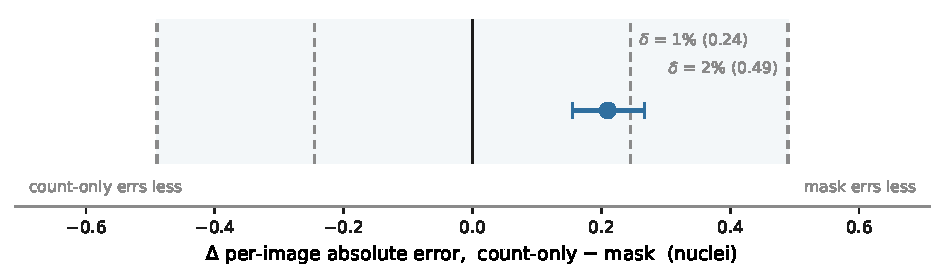
\includegraphics[width=0.85\textwidth]{fig_equivalence.pdf}
\caption{Per-image difference in absolute error between the two supervision regimes on PanNuke fold~3
($n=2722$), with a $90\%$ bootstrap confidence interval, shown against equivalence margins $\delta$ expressed
as a fraction of the mean nuclei per image. The confidence interval excludes $0$, so the difference is real;
at the same time it lies entirely within the $2\%$ margin, so the difference is bounded above at that level.
The smallest margin still yielding equivalence is $\delta^\star = 0.27$ nuclei.}
\label{fig:equivalence}
\end{figure}

The scope of this comparison should be noted: the mask branch uses the \emph{same} architecture as count-only
in order to isolate the effect of \emph{supervision type}, so it does not measure the capability of a
purpose-built segmentation architecture. Section~\ref{sec:paradigm} addresses that question separately.

\subsection{What evidence does a count-only model rely on?}\label{sec:fidelity}

The results in Section~\ref{sec:parity} show that removing spatial supervision changes counting accuracy only
within a narrow margin on the largest dataset, but they do not say what evidence the model uses to count. A
model that sees only one number per image could in principle exploit global correlates (tissue type, cellular
density, staining characteristics) rather than the nuclei themselves. The two analyses below test that
possibility on PanNuke fold~3 ($n=2722$ patches, mean count $24.5$).

\paragraph{Accuracy is retained across all 19 tissue types.} The analyses below use three independently trained
count-only models following the protocol in Section~\ref{sec:setup}, from a training run separate from the
models of Table~\ref{tab:parity}; the model used for Table~\ref{tab:perorgan} and Fig.~\ref{fig:agreement}
attains $R^2 = 0.934$ and MAE $3.40$ over the whole test set. Predictions lie close to the line of exact
counting across the full range of counts (Fig.~\ref{fig:agreement}a). Broken down by tissue type
(Table~\ref{tab:perorgan}), $R^2$ is positive in \emph{all} $19/19$ types, ranging from $0.704$ (Ovarian,
$n=52$) to $0.976$ (Cervix, $n=86$). The two lowest values fall on tissue types with few test patches, where
the $R^2$ estimate is less stable, but the relationship is not monotone: the tissue type with the fewest
patches (Pancreatic, $n=28$) still attains $0.901$, while the third-lowest value belongs to a well-represented
type (Adrenal gland, $n=155$, $R^2 = 0.818$). Bland--Altman analysis gives a bias of $+0.70$ nuclei, about
$3\%$ of the mean count, with limits of agreement of $\pm10.2$ nuclei (Fig.~\ref{fig:agreement}b), meaning that
the error carries no systematic directional bias. Overall accuracy therefore does not come from fitting a few
majority tissue types well.

\begin{figure}[!htbp]
\centering
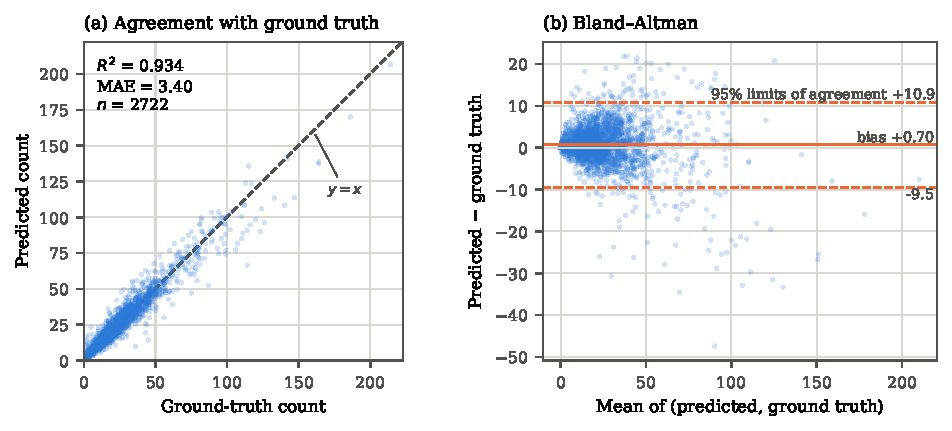
\includegraphics[width=\textwidth]{fig_agreement.pdf}
\caption{Agreement between predicted and ground-truth nuclei counts for the count-only model on PanNuke fold~3
($n=2722$ patches). \textbf{(a)} Each point is one patch; the dashed line is exact counting.
\textbf{(b)} Bland--Altman plot with mean bias and $95\%$ limits of agreement. The downward spread at
high-count patches indicates a mild tendency to \emph{under-count} in the very high density regime.}
\label{fig:agreement}
\end{figure}

\begin{table}[!htbp]
\centering
\caption{Counting accuracy per tissue type on PanNuke fold~3, for \emph{one} of the three count-only models of
Section~\ref{sec:fidelity} (Fig.~\ref{fig:agreement} plots the same model), the overall row included.
Table~\ref{tab:parity} reports seed-aggregated figures from a different training run, so the two overall rows
do not coincide.}\label{tab:perorgan}
\small
\setlength{\tabcolsep}{4pt}
\begin{tabular}{@{}lccc@{\hspace{1.5em}}lccc@{}}
\toprule
Tissue type & $n$ & $R^2$ & MAE & Tissue type & $n$ & $R^2$ & MAE \\
\midrule
Adrenal gland & $155$ & $0.818$ & $2.43$ & Lung       & $51$  & $0.957$ & $3.61$ \\
Bile duct     & $158$ & $0.942$ & $2.71$ & Ovarian    & $52$  & $0.704$ & $4.31$ \\
Bladder       & $64$  & $0.924$ & $2.34$ & Pancreatic & $28$  & $0.901$ & $3.29$ \\
Breast        & $775$ & $0.932$ & $2.65$ & Prostate   & $68$  & $0.756$ & $4.43$ \\
Cervix        & $86$  & $0.976$ & $2.20$ & Skin       & $41$  & $0.943$ & $5.72$ \\
Colon         & $494$ & $0.923$ & $3.93$ & Stomach    & $48$  & $0.963$ & $3.95$ \\
Esophagus     & $141$ & $0.897$ & $3.19$ & Testis     & $57$  & $0.949$ & $3.05$ \\
Head \& neck  & $145$ & $0.954$ & $3.17$ & Thyroid    & $62$  & $0.873$ & $3.30$ \\
Kidney        & $41$  & $0.958$ & $4.51$ & Uterus     & $163$ & $0.907$ & $6.70$ \\
Liver         & $93$  & $0.884$ & $3.39$ & \textbf{Overall} & $2722$ & $0.934$ & $3.40$ \\
\bottomrule
\end{tabular}
\end{table}

\paragraph{Sham-controlled nucleus removal.} To test the causal relationship, a fraction $k$ of the annotated
nuclei is removed from the image and the predicted count is measured again. Each nucleus is replaced by a
\emph{shape-matched} tissue patch taken from a nucleus-free location within the same image, and the nucleus
mask is dilated by $2$ pixels before removal so as to cover the nuclear rim that annotation commonly omits.
This operation preserves the texture statistics of the tissue while removing nuclear content. The sham control
applies \emph{exactly} the same operation with the same number of regions, the same shapes and the same area,
but at nucleus-free locations. It separates the effect of the tissue replacement itself from the effect of
losing nuclei. Only measurements whose removed areas match to at least $80\%$ between the two conditions enter
the statistical tests.

\begin{figure}[!htbp]
\centering
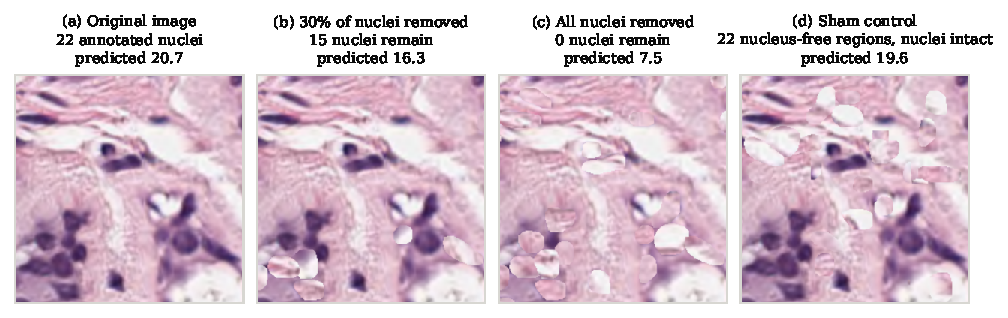
\includegraphics[width=\textwidth]{fig_qualitative.pdf}
\caption{Nucleus removal on a representative PanNuke patch (its own response coefficient is $0.65$ against the
dataset mean of $0.64$). \textbf{(a)} Original image, $22$ annotated nuclei. \textbf{(b, c)} After removing
$30\%$ and then all annotated nuclei, the predicted count falls accordingly
($20.7 \rightarrow 16.3 \rightarrow 7.5$). \textbf{(d)} Sham control on $22$ \emph{nucleus-free} regions: the
image is visibly manipulated, yet the count is almost unchanged ($19.6$). The few dark nuclei remaining in (c)
are nuclei absent from the annotation.}
\label{fig:qualitative}
\end{figure}

The predicted count falls \emph{monotonically} with the fraction of nuclei removed, while the sham control
leaves the count essentially unchanged ($1.00$--$1.02$) at every level (Table~\ref{tab:doseresp};
Fig.~\ref{fig:qualitative} illustrates the operation on one patch). Over the area-matched measurements
($n=3415$), the drop attributable to nuclei is $0.234$ normalised units and accounts for the entire observed
drop (paired Wilcoxon between the two conditions, $p<10^{-300}$). The conclusion is unchanged when only the
small doses ($\le 30\%$) are considered, where the images remain closest to the training distribution. The
response is therefore \emph{specific} to nuclei rather than to image manipulation as such.

\begin{table}[!htbp]
\centering
\caption{Response of the predicted count to nucleus removal, against a sham control that removes an equal area
of nucleus-free tissue. Values are normalised by the count on the intact image, averaged over $286$ images
($4862$ measurements) and then over $3$ independently trained models; the reported standard deviation is the
deviation across those three models. The ``response coefficient'' is the observed drop divided by the drop of a
faithful tallying counter; a value of $1.0$ corresponds to faithful tallying.}\label{tab:doseresp}
\footnotesize
\setlength{\tabcolsep}{5pt}
\begin{tabular}{@{}cccccc@{}}
\toprule
Fraction removed & Nucleus removal & Sham & Attributable drop & Area match & Response coeff. \\
\midrule
$10\%$  & $0.938\pm0.002$ & $1.003$ & $0.065$ & $0.94$ & $0.62$ \\
$20\%$  & $0.872\pm0.004$ & $1.004$ & $0.131$ & $0.91$ & $0.64$ \\
$30\%$  & $0.805\pm0.012$ & $1.007$ & $0.202$ & $0.89$ & $0.65$ \\
$50\%$  & $0.678\pm0.014$ & $1.011$ & $0.333$ & $0.84$ & $0.64$ \\
$75\%^{\ast}$  & $0.519\pm0.020$ & $1.012$ & $0.494$ & $0.78$ & $0.64$ \\
$100\%^{\ast}$ & $0.374\pm0.051$ & $1.018$ & $0.644$ & $0.73$ & $0.63$ \\
\bottomrule
\end{tabular}

\vspace{4pt}
\begin{minipage}{\textwidth}\footnotesize
$^{\ast}$ At high doses, nucleus-dense histopathology no longer leaves enough free space to place
non-overlapping sham regions, so the removed areas of the two conditions match only to $0.74$--$0.78$; these
levels are reported descriptively and excluded from the statistical tests, which use only measurements with at
least $80\%$ area match. In addition, removing all nuclei intervenes on ${\sim}25\%$ of the image area and thus
induces a substantial distribution shift; the small doses are therefore treated as the primary evidence.
\end{minipage}
\end{table}

The response is, however, consistently \emph{sublinear}: the ratio between the observed drop and the drop of a
faithful tallying counter lies between $0.62$ and $0.65$ at \emph{every} dose from $10\%$ to $100\%$ (last
column of Table~\ref{tab:doseresp}), and averages $0.64 \pm 0.04$ over the three independently trained models.
Removing one nucleus lowers the count by about $0.6$ rather than $1.0$. This shortfall is a fixed coefficient,
not a saturation effect at high doses.

The most consistent interpretation is that the model \emph{integrates nucleus-related evidence over the whole
image} rather than detecting and tallying individual instances. An independent measurement supports this
reading: the density map of the count-only model \emph{barely} localises nuclei. The density mass falling
inside true nuclear regions is only $1.25\pm0.36$ times that of a uniform map ($1.0$ corresponding to no
localisation at all), so the departure from the no-localisation baseline is smaller than the between-seed
variation; and the spatial correlation with the ground-truth density map is only $0.03$ (three seeds), close to
chance. The reference point here is a map carrying no positional information, not the localisation ability of a
densely supervised model, which is not measured in this paper. The two observations are consistent with a
single explanation, and it accounts for why image-level supervision suffices for \emph{counting} without giving
rise to localisation ability: the supervised quantity is a sum, so the solution the model finds need only be
correct at the level of the sum.

Three additional checks show that this shortfall is not an artefact of how removal was designed; all three run
on \emph{one} count-only model, so they should be read as differences between configurations. First, dilating
the mask by $0$, $2$ and $4$ pixels before removal, corresponding to intervened areas of $18\%$, $25\%$ and
$31\%$ of the image, gives coefficients of $0.59$, $0.60$ and $0.61$; this entire range is smaller than the
deviation between models, so incomplete coverage of the nuclear rim does not explain the shortfall. Second,
nuclei missed by the annotation are not removed and therefore still contribute to the count: the residual count
after removing all annotated nuclei rises monotonically from $0.36$ on patches with no sign of missed nuclei to
$0.70$ in the group with the most missed nuclei (correlation $+0.31$, $n = 286$), but the portion of the
prediction exceeding the annotated count averages only about $3.5\%$ against a residual count of $37.4\%$, so
most of the gap to $1.0$ cannot be attributed to annotation quality. Conversely, the measurement \emph{is}
sensitive to how the removed region is filled: replacing patch transplantation with Telea inpainting at the
same dilation drops the coefficient from $0.59$ to $0.34$, because inpainting propagates colour inward from the
boundary of the region to be filled, and that boundary is the nuclear rim itself, so it leaves a nuclear trace
in the image. The measured coefficient is therefore capped by how complete the removal is, and $0.64$ is a
lower bound on the true sensitivity.

\subsection{Comparison with methods that use localisation labels}\label{sec:paradigm}

The lightweight count-only counter attains better $R^2$ and MAE than all three surveyed representatives of
segmentation, density estimation and detection, despite using only count labels (Table~\ref{tab:paradigm}).
Each paradigm is represented by \emph{one} method, so this result speaks to the specific methods surveyed and
not to the limits of an entire approach. All four methods are retrained and evaluated on the same test set at
the level of the counting task. The count of each compared method is obtained through that method's own
official post-processing: the number of instances after splitting for StarDist, the number of local maxima on
the centroid density map for DualU-Net, and the number of points surviving non-maximum suppression for DeNuC.
Unlike the controlled comparison in Section~\ref{sec:parity}, architecture, parameter count and
hyperparameters all differ between the methods here, so the result indicates how these paradigms behave in
their common configurations on the counting task rather than isolating a single cause.

The detection method degrades monotonically with nuclear density: the count bias grows from $-0.8$ on sparse
patches to $-30.4$ on patches with $45$ or more nuclei. This progression matches the mechanism by which
non-maximum suppression discards true positives when nuclei overlap, and explains why count regression
dominates in the high density regime.

\begin{table}[!htbp]
\centering
\caption{Comparison of four paradigms on PanNuke (same test set, counting task). DensitySigmaUNet reports the
mean and standard deviation over $5$ seeds, the same figures as in Table~\ref{tab:parity}; the three compared
methods are a single training run each, so differences between them should be read against the level of
between-seed variation shown in its row. The best value in each column is in bold.}\label{tab:paradigm}
\small
\begin{tabular}{@{}lccccc@{}}
\toprule
Method & Params & Labels & Paradigm & $R^2\uparrow$ & MAE$\downarrow$ \\
\midrule
DensitySigmaUNet & $3.62$M & counts & regression & $\mathbf{0.918\pm0.011}$ & $\mathbf{3.60\pm0.10}$ \\
StarDist~\cite{stardist} & $1.43$M & masks & segmentation & $0.841$ & $4.64$ \\
DualU-Net~\cite{dualunet} & $41.0$M & masks & centroid density & $0.804$ & $5.33$ \\
DeNuC~\cite{denuc} & $4.37$M & points & detection & $0.455$ & $9.64$ \\
\bottomrule
\end{tabular}
\end{table}

\subsection{The system against its three budgets}\label{sec:deploy}
\subsubsection{Annotation budget}\label{sec:label}
One quarter of the annotation budget already suffices for about $93\%$ of the performance obtained with full
labels. On PanNuke, $R^2$ as a function of the fraction of count-labelled images is $0.453 \pm 0.208$ at $5\%$,
$0.742$ at $10\%$, $0.849 \pm 0.029$ at $25\%$, $0.859$ at $50\%$ and $0.915 \pm 0.010$ with all labels (three
seeds, same evaluation protocol; the full-budget value differs by $0.003$ from Table~\ref{tab:parity}, within
the between-seed variation). The curve saturates early: most of the gain is realised within the first quarter
of the budget, while going from $25\%$ to $100\%$ adds only $0.066$. The $5\%$ point marks the lower limit of
this regime, where the between-seed variance dominates the mean. For a deployment this means that the
annotation contract can be sized well below full coverage, and that the marginal value of each additional
labelled image is measurable in advance rather than assumed.

\subsubsection{Annotation cost per label type and compute budget}\label{sec:cost}
The larger difference lies on the annotation side. Qu et al.~\cite{qu2020} had a pathologist annotate eight
images in three different ways and measured the time: for images containing about $600$ nuclei on average, full
delineation took about $115$ minutes, bounding boxes about $67$ minutes, and placing a point on every nucleus
only about $14$ minutes. The cost of image-level count labels has not been measured directly in the
literature, but it is bounded above by the cost of point marking: counting requires scanning the nuclei exactly
as point marking does, without having to place each point precisely and without any delineation. On those
figures, count labels are at least $8$ times cheaper than full masks, and an approximate count is cheaper
still. This ratio should be read as an order of magnitude rather than a transferable constant: it rests on
eight images from a single annotator, and those images are far denser than the $256\times256$ patches used
here (mean $24.5$ nuclei). What is preserved between the two regimes is the cost \emph{per nucleus}: on the
same figures, delineation costs about $11.5$ seconds per nucleus and point marking about $1.4$ seconds, and
counting cannot be more expensive than marking. Set against the loss of accuracy measured in
Section~\ref{sec:parity}, bounded above by roughly $1\%$ of the nuclei per image, this asymmetry is the central
efficiency argument of the paper.

On the compute side the counter has $3.62$M parameters and $0.98$ GMACs at $256\times256$ input, a latency of
$6.0$\,ms on GPU and $46$\,ms on CPU, and a peak memory of $37.9$\,MB. These figures permit real-time inference
on both commodity GPUs and CPUs, so the deployed system does not require dedicated accelerator hardware. The
comparison in Table~\ref{tab:paradigm} shows that this is not obtained by trading accuracy for size: the
counter is $11.3$ times smaller than the largest compared method and still more accurate on the counting task.

\subsubsection{Reliability specification}\label{sec:uq}
The prediction intervals are calibrated not only marginally but also conditionally on organ
(Table~\ref{tab:uq}). All three schemes reach the target marginal coverage of $0.90$, but only mondrian raises
the coverage of the worst-covered organ to that same target ($0.906$), whereas a single shared threshold leaves
four of the $19$ tissue types below the tolerance threshold. The price is an interval about $15\%$ wider. This
distinction is what turns an average-case number into a usable specification: a system whose stated tolerance
holds overall but fails on four tissue types out of nineteen cannot be certified for those tissues, and the
$15\%$ width penalty is the cost of removing that failure mode.

The observed coverages are not free parameters: all three follow from Eq.~\eqref{eq:cov} and the sizes of the
calibration groups, with nothing fitted. The calibration half of fold~3 holds $n = 1361$ images, giving a
predicted global coverage of $k/(n+1) = 0.901$ against $0.904$ observed. Under the mondrian scheme the same
images are split by organ into groups of $n_g = 14$ (Pancreatic) to $387$ (Breast); the single group below the
threshold of $15$ falls back on the global $q$, and the size-weighted average of $k_g/(n_g+1)$ over the
remaining eighteen is $0.919$, against $0.923$ observed. For the cluster scheme the three pooled groups are
large enough that the prediction is $0.903$ regardless of which organs are pooled together, varying by less
than $0.001$ over every possible assignment of the nineteen organs to three groups, against $0.906$ observed.
Each prediction is therefore within $0.004$ of the measurement, and the residual is positive in all three
cases, as expected: the interval is truncated below at zero and the scores are ties-prone because counts are
integers, and both effects can only raise coverage above the bound in Eq.~\eqref{eq:cov}.

This is the sense in which the over-coverage of mondrian, $0.923$ against a target of $0.90$, is not a defect
of calibration but the price of the conditional guarantee. Splitting $1361$ calibration images into nineteen
organ groups makes the $1/(n_g+1)$ slack of Eq.~\eqref{eq:cov} roughly nineteen times larger, and it is that
slack, not a miscalibrated $\sigma$, which produces both the extra coverage and the $15\%$ extra width. The
quantity a deployment buys with that width is the last column of Table~\ref{tab:uq}.

Anchoring $\sigma$ to a Poisson variance baseline matters when the range of counts is wide. On NuInsSeg, where
the per-image count spans from a few nuclei to more than $500$, the Poisson-anchored form gives an interval
width of $37.7$ against $67.9$ for an unanchored $\sigma$ ($-44\%$), a Winkler score of $45.4$ against $78.1$
($-42\%$), and a worst-organ coverage of $0.864$ against $0.655$, at the same marginal coverage of
${\sim}0.93$. On PanNuke, where the counts are concentrated in a narrow range, the two forms do not differ
appreciably. Poisson anchoring is therefore a design choice for wide-range data rather than a uniform
improvement. The $\sigma$ head does not reduce counting accuracy, because $\mu$ is detached from the
uncertainty branch.

\begin{table}[!htbp]
\centering
\caption{Prediction interval quality after conformal calibration on PanNuke fold~3 ($n=2722$), averaged over
$20$ random calibration splits. The target coverage is $0.90$; width and Winkler score are in units of nuclei,
lower being better. A tissue type counts as under-covered when its coverage falls more than $0.05$ below the
target, that is below $0.85$; this tolerance explains why the cluster scheme has a worst-organ coverage of
$0.859$ and yet no tissue type counted as under-covered. The best value in each column is in bold, except for
marginal coverage, which is a validity check against the $0.90$ target rather than a quantity to be
maximised.}\label{tab:uq}
\footnotesize
\setlength{\tabcolsep}{5pt}
\begin{tabular}{@{}lccccc@{}}
\toprule
Scheme & Marginal coverage & Width & Winkler & Worst-organ coverage & Under-covered \\
\midrule
global & $0.904$ & $\mathbf{14.5}$ & $20.3$ & $0.765$ & $4/19$ \\
mondrian & $0.923$ & $16.6$ & $20.5$ & $\mathbf{0.906}$ & $\mathbf{0/19}$ \\
cluster & $0.906$ & $14.8$ & $\mathbf{20.0}$ & $0.859$ & $\mathbf{0/19}$ \\
\bottomrule
\end{tabular}
\end{table}

%%============================================================%%
\section{Discussion}\label{sec:discuss}

\paragraph{Why image-level supervision can suffice for nuclei counting.} The intervention experiments offer a
plausible explanation for why detailed positional information is not the decisive component of counting
accuracy. The predicted count falls specifically when nuclei are removed from the image but barely changes
under area-matched sham interventions; at the same time, the response remains sublinear and the learned density
map carries almost no positional information. These two observations are consistent with the hypothesis that
the model learns to integrate nucleus-related evidence over the whole image rather than to detect and tally
individual instances. In that case, an image-level count label may already provide most of the information
needed for the counting task.

\paragraph{Design implications.} Read against the three budgets of Section~\ref{sec:intro}, the measurements
give a system that is cheap on all three axes at once. The annotation contract can be written for image-level
counts, at least eight times cheaper per image than full delineation, and sized at roughly a quarter of full
coverage for about $93\%$ of the attainable accuracy. The inference cost stays within what a CPU can serve in
real time, so the system does not impose accelerator hardware on the site that deploys it. The reliability
requirement is met by organ-conditional conformal calibration, which is a post-hoc procedure and therefore does
not constrain how the counter itself was trained. The single quantity to be traded away is bounded above by
roughly $1\%$ of the nuclei per image on the largest dataset tested. This asymmetry, rather than any individual
accuracy figure, is what makes the count-only design the rational choice when the required output is the count.

\paragraph{Out-of-domain transfer.} The whole-image evidence integration mechanism also suggests a potential
limitation. Because the model learns nucleus-related signals at a particular spatial scale, accuracy may
degrade when magnification or apparent nuclear size differs substantially between the training and deployment
domains. Conformal prediction intervals, by contrast, assume no particular distributional form: after
recalibration on a small calibration set from the target domain, the desired coverage is maintained under
exchangeability even if point accuracy changes. Widening intervals then act as a warning signal that a sample
lies outside the region where the model remains trustworthy.

\paragraph{Limitations and scope.} This study was designed as a controlled experiment isolating the role of
supervision type. Its conclusions are therefore established on a single architecture family, a lightweight
encoder combined with a U-Net style decoder. Whether similar observations continue to hold on other
architectures, such as transformer models or purpose-built nuclei segmentation systems, remains to be verified
empirically. Also, because the mask branch uses the counter's own architecture, the main comparison measures
the role of \emph{supervision type} and does not establish an upper bound for a separately optimised
segmentation pipeline; Section~\ref{sec:paradigm} only partly fills that gap.

In addition, this paper considers only the counting task. The results do not imply that image-level supervision
suffices for tasks requiring spatial information, such as instance segmentation, nucleus localisation or
morphological analysis. On the contrary, the intervention results indicate that a count-only model does not
readily form a meaningful localised representation, even when it counts accurately.

\section{Conclusion}\label{sec:conclusion}

This paper tested the role of spatial supervision in nuclei counting directly, through a controlled experiment
in which architecture, data and evaluation protocol were held fixed and the only variable was the type of
supervision. Across three independent histopathology datasets neither regime is consistently superior; on
PanNuke, the advantage of mask supervision is statistically significant but bounded above by an equivalence
test at roughly $1\%$ of the mean nuclei per image. Image-level count labels, meanwhile, are at least eight
times cheaper than full delineation.

The intervention experiments show that the count-only model responds specifically to nuclear content but forms
its prediction by integrating evidence over the whole image rather than by localising individual instances,
which both explains the counting accuracy attained and marks its limits for tasks that require spatial
information. On the counting task itself, the counter attains higher accuracy than all three surveyed
representatives of methods that use localisation labels, runs in real time on a CPU, and carries
organ-conditional prediction intervals that hold their target coverage in every tissue type.

Overall, for nuclei counting, dense spatial annotation is not a prerequisite for high accuracy, and the
annotation budget of a deployed quantification system can be reduced by roughly an order of magnitude for a
bounded and measurable loss. Future directions include verifying how far this conclusion generalises to other
architecture families and to data domains differing substantially in resolution, organ and staining protocol;
and tracing which image features constitute the integration the counter learns, including the question of why
its response coefficient is below one.

%%============================================================%%
\section*{CRediT authorship contribution statement}
\textbf{Viet Hang Duong:} Conceptualisation, Methodology, Validation, Writing -- review and editing,
Supervision. \textbf{Thi Thu Hiep Dinh:} Conceptualisation, Investigation, Software, Formal analysis,
Visualisation, Writing -- original draft.

\section*{Declaration of competing interest}
The authors declare that they have no known competing financial interests or personal relationships that could
have appeared to influence the work reported in this paper.

\section*{Declaration of generative AI and AI-assisted technologies in the writing process}
%% RINENG/Elsevier bat buoc muc nay NEU co dung AI ho tro viet. Neu khai, phai khai dung.
%% Neu quyet dinh khong khai, XOA CA MUC nay, dung de trong.
During the preparation of this work the authors used AI-assisted tools in order to improve the readability and
language of the manuscript. After using these tools, the authors reviewed and edited the content as needed and
take full responsibility for the content of the publication.

\section*{Funding}
This research was funded by the VNUHCM-University of Information Technology's Scientific Research Supported
Fund.

\section*{Ethics approval}
Not applicable. The study uses only publicly available, previously published and de-identified histopathology
image datasets; no new data were collected from human participants or animals.

\section*{Data availability}
The study uses publicly available data only: PanNuke~\cite{pannuke}, NuInsSeg~\cite{nuinsseg} and
MoNuSeg~2018~\cite{monuseg}, accessible through their respective original publications. No new data were
generated. The code used to train, evaluate and reproduce every table and figure in this article will be made
publicly available upon acceptance.

\section*{Acknowledgements}
The authors thank the VNUHCM-University of Information Technology for supporting this research.

\bibliographystyle{elsarticle-num}
\bibliography{references}

\end{document}
